\documentclass[main.tex]{subfiles}
\begin{document}

\subsection*{Introduction}

\marginpar{Monday\\ 2021-11-8, \\ compiled \\ \today}

This first part of this course is given by Ivan De Mitri. 

This is not a course on particle detectors: the basics will be assumed, and there will be some short courses about the details. 
It is more about ``experimental tools'': how do we design an experiment? 

``High energy'', here, means roughly considering energies \(E \gtrsim \SI{1}{GeV}\), but there will be some things in the \SI{}{MeV} range as well. 
A more apt description of this field is that it is about observing things that come from outside the Earth: particles or high-energy radiation. 

The other, ``low-energy'' course is about the search for rare events, where the issue is the presence of a large background, so we need to go underground. 

Then, there is neutrino physics which is at the intersection between these two areas. 

The part on gravitation and cosmology, on the other hand, is wholly distinct. 

\subsubsection*{Cosmic rays}

We start with a review of some basic concepts. 

As a first approximation, the spectrum of cosmic particles/radiation \(\phi (E)\) is decreasing with \(E\). 
From \(E \sim \SI{e8}{eV}\) to \(E \sim \SI{e20}{eV}\) there is roughly a powerlaw, \(\phi \propto E^{-\gamma }\) with \(\gamma \sim 2.7\) at first, then \(\gamma \sim 3\) (as shown in figure \ref{fig:cosmic_rays_energies}). 

With artificial particle accelerators we can probe up to roughly \SI{e13}{eV} (since in the center of mass we have \((7 + 7) \SI{}{TeV}\)). 

% The way to explore the \SI{}{eV} energy range is completely different from big particle colliders: this is a general fact, the way to explore the low energy region is different from the high energy region. 

Since the spectrum is roughly a power-law with index 3 spanning 12 orders of magnitude,
the number of observed events changes by roughly \(12 \times 3\) orders of magnitude between its ends. 

There is a ``knee'' in the energy spectrum, where the spectral index \(\gamma\) goes from 2.7 to 3, is at about \SI{3e15}{eV}. 

\begin{figure}[ht]
\centering
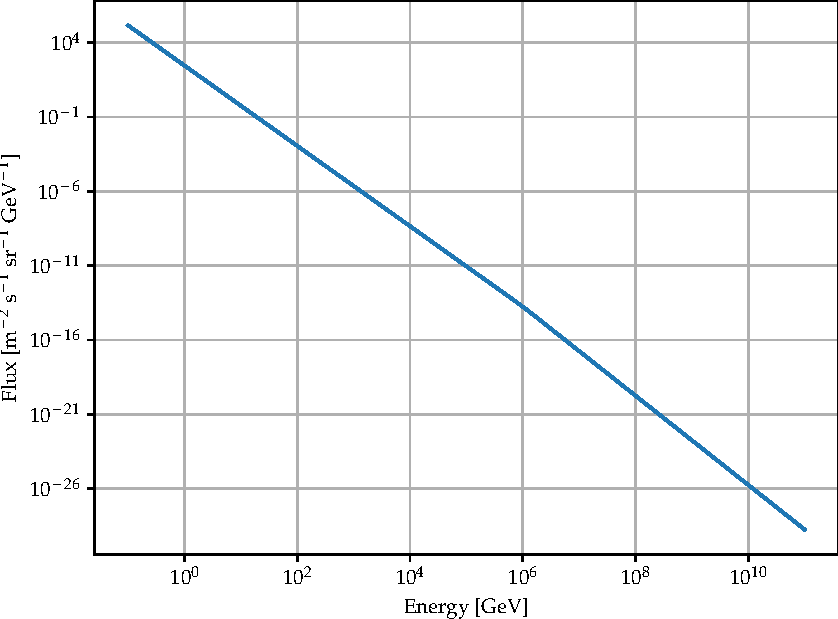
\includegraphics[width=\textwidth]{figures/cosmic_rays_energies}
\caption{A rough sketch of the cosmic ray flux dependence on the energy.}
\label{fig:cosmic_rays_energies}
\end{figure}

Typically, below the knee we can do direct, small experiments, while above it we need to do indirect measurements: they need to be very large, since the presence of a single event becomes very rare.

The particles which have been found to make up \textbf{cosmic rays} are protons \ce{p}, Helium nuclei \ce{He}, heavy nuclei such as \ce{Fe}, \(\gamma \) rays, electrons and positrons \(e^{\pm}\), antiprotons \(\ce{\overline{p}}\). 
Anti-helium still has to be discovered, but there has been some progress in this regard lately. 

Also, there are neutrinos: solar ones are on the scale of the \SI{}{MeV}, up to \SI{10}{MeV}. 
Protons come down the atmosphere and interact with it a few tens of \SI{}{km} above, producing other things, such as neutrinos (these are ``atmospheric neutrinos'').
Alternatively, we can have a source producing neutrinos directly, ``astrophysical neutrinos''. 

\emph{Why} are we doing these experiments?
\begin{enumerate}
    \item We can explore the astrophysical processes allowing for the production of such high-energy particles, and
    \item we can probe high-energy particle physics. 
\end{enumerate}

In order to match the center-of-mass energy of the LHC collisions we'd need to have \SI{e17}{eV} in a fixed-target experiment.

This is due to the fact that fixed-target experiments have much lower center-of-mass energetics in general. 

Here is a quick sketch of why, in natural units, using the formalism detailed in the second half of this lecture.
If we have two particles colliding and with equal and opposite momenta the total four-momentum will be \(p _{\text{tot}} = (E, \vec{p}) + (E, - \vec{p}) = (2E, \vec{0})\), therefore the total center-of-mass energy will be \(\sqrt{s} = 2 E\).

On the other hand, in a fixed-target experiment we will have one of them being stationary, so the total four-momentum will be \(p _{\text{tot}} (E, \vec{p}) + (m, \vec{0}) = (E+m, \vec{p})\), where the momentum \(\vec{p}\) is determined by \(m^2 = E^2 - m^2\), so the magnitude will be \(\sqrt{s} = \sqrt{(E+m)^2 - (E^2 - m^2)} = \sqrt{2m (E+m)}\). 

In terms of the Lorentz factor \(\gamma \) the beam-beam collision is \(\sqrt{s} = 2 m \gamma \), while the fixed-target one is \(\sqrt{s} = m\sqrt{2(1+\gamma )}\). For large values of \(\gamma \), the first one clearly wins out, by a factor roughly \(\sqrt{\gamma }\).

Specifically, if one wants \(\sqrt{s} = \SI{14}{TeV}\), this can be achieved with \(E \approx \SI{7}{TeV}\) in a beam-beam collision, or with \(E \approx \SI{1000}{TeV}\) in a fixed-target collision. 
The ratio, as expected, is roughly \(70 \divisionsymbol 80 \approx \sqrt{\gamma } = \sqrt{\SI{7}{TeV} / \SI{1}{GeV}}\) when accounting for the fact that we need to accelerate twice as many particles in the beam-beam scenario.

\subsubsection*{History}

Cosmic rays were discovered in the early 1900s, and up to the early 50s most particle physics was done through them.

In 1957 the antiproton was discovered by Segrè and Chamberlain.
This was done with accelerators, thanks to proton collisions producing secondaries, in a process like 
%
\begin{align}
\ce{p} + \ce{A} \to \ce{p} + \ce{A} + \ce{p} + \ce{\overline{p}}
\,.
\end{align}
%
 
The cosmic ray discovery of the antiproton was performed only a few months later. 

% In the early days the approach was to be ``particle 
% hunters'', then people became ``particle breeders''. 

\subsubsection*{References}

A good one is \textcite{aloisioSelectedTopicsCosmic2018}.

\section{Review}

\subsection{Relativistic kinematics}

Suppose we have a frame \(O\) and a different frame \(O'\) moving with constant velocity along the \(x \sim x'\) direction. 

If we define, in terms of the speed of light \(c\) and the relative velocity \(v\) between the two frames,
%
\begin{align}
\beta  = \frac{\abs{\vec{v}}}{c} \qquad \text{and} \qquad
\gamma = \frac{1}{\sqrt{1 - \beta^2}}
\,,
\end{align}
%
then all observations in one frame can be connected with ones in the other thanks to the Lorentz transformation law. 

The way the four-vector \((ct, x, y, z)^{\top}\) transforms is 
%
\begin{align}
\left[\begin{array}{c}
ct' \\ 
x' \\ 
y' \\ 
z'
\end{array}\right]
= \left[\begin{array}{cccc}
\gamma  & -\gamma \beta  & 0 & 0 \\ 
-\gamma \beta  & \gamma  & 0 & 0 \\ 
0 & 0 & 1 & 0 \\ 
0 & 0 & 0 & 1
\end{array}\right]
\left[\begin{array}{c}
ct \\ 
x \\ 
y \\ 
z
\end{array}\right]
\,.
\end{align}

This is actually a general law, since we can write the transformation decomposing the position vector into parallel and perpendicular components to the motion: 
%
\begin{align}
\left[\begin{array}{c}
ct' \\ 
r_{\parallel}'
\end{array}\right]
&=
\left[\begin{array}{cc}
\gamma  & -\gamma \beta  \\ 
-\gamma \beta  & \gamma 
\end{array}\right]
\left[\begin{array}{c}
ct \\ 
r_{\parallel}
\end{array}\right]  \\
r'_{\perp} &= r_{\perp}
\,.
\end{align}

We can denote \((ct, x, y, z)^{\top}\) as \((x_0, x_1, x_2, x_3 ) \equiv x\). 

The scalar product used by these vectors is the mixed signature 
%
\begin{align}
x \cdot y = x^{\mu } \eta_{\mu \nu } x^{\nu }
\,,
\end{align}
%
where
%
\begin{align}
\eta_{\mu \nu } = \left[\begin{array}{cccc}
1 & 0 & 0 & 0 \\ 
0 & -1 & 0 & 0 \\ 
0 & 0 & -1 & 0 \\ 
0 & 0 & 0 & -1
\end{array}\right]
\,,
\end{align}
%
because we are using the evil particle physicist's mostly-minus convention.

We choose this because of the invariance of the spacetime interval. 

Lorentz transformations are ``rotations'' in the sense that they leave the magnitude of vectors unchanged. 

We need to define a \emph{velocity} four-vector.
In the nonrelativistic case, \(\vec{v} = \dv*{\vec{r}}{t}\); how do we extend it to the relativistic case?

We could define this as \(\dv*{x_{\mu }}{t}\), but this is not invariant since time is not invariant (i.e.\ it is not a scalar).

Instead, we define the \emph{proper time} as the time \emph{as measured in the reference frame of the particle}. 
We know that \(\Delta t = \gamma \Delta \tau \) by the Lorentz transformation law: therefore, we can define the relativistic velocity as
%
\begin{align}
u_{\mu } = \lim_{ \Delta \tau \to 0} \frac{ \Delta x_{\mu }}{\Delta \tau } = \gamma \dv{x_{\mu }}{t}
\,.
\end{align}

This is indeed a four-vector.
Its components are \((\gamma c, \gamma v_x, \gamma v_y, \gamma v_z)^{\top}\), where \(\vec{v}\) is the non-relativistic velocity \(\dv*{\vec{x}}{t}\). 

The magnitude of this four-vector must be a Lorentz invariant: it comes out to be 
%
\begin{align}
u^2 = \gamma^2 \qty(c^2 - \abs{v}^2) = c^2
\,.
\end{align}

In the nonrelativistic case the momentum is \(\vec{p} = m \vec{v}\), while in the relativistic case we can define \(p = m u\). 

Its components will be 
%
\begin{align}
p^{\mu } = (\gamma m c, \gamma m \vec{v})^{\top}
\,.
\end{align}

The term \(\gamma mc\) is the (kinetic + rest) energy divided by the speed of light: 
%
\begin{align}
\gamma mc &= \frac{mc}{\sqrt{1 - \beta^2}} \approx mc \qty(1 - \frac{1}{2} \beta^2)  \\
&\approx \frac{1}{c} \qty(mc^2 + \frac{1}{2} mv^2 + \order{\beta ^{4}})
\,.
\end{align}

Therefore, we can write \(p = (E/c, \vec{p})^{\top}\), where \(\vec{p} = \gamma m \vec{v}\) and \(E = \gamma m c^2\). 
This is a four-vector, and transforms as such, since the mass is a scalar. 
Its magnitude is \(p^2 = m^2 c^2\). 
This relation means that 
%
\begin{align}
E^2 = (mc^2)^2 + (\abs{p}^2 c^2)^2
\,.
\end{align}

The conventional way to define the kinetic energy is \(E _{\text{kin}} = E - mc^2\). 

If we have a system of particles with four-momenta \(p_i\) we can compute the total energy and the total three-momentum by adding them all together. 

If these particles scatter the four-momentum is conserved. 
What is the variable associated with the modulus of the total momentum? 
%
\begin{align}
p _{\text{tot}}^2 = \qty(\frac{\sum _{i} E_i}{c})^2 - \abs{\sum _i \vec{p}_i}^2 \overset{\text{def}}{=} M^2 c^2s
\,.
\end{align}

The variable \(M\) is called \emph{invariant mass}, and it is also written in terms of the Mandelstam variable \(s\) as \(\sqrt{s}\) in the case of a two-two process.

\subsection{The \(J/\psi \) discovery}

Professor Samuel Ting got the Nobel Prize in 1976. 
His experiments can be used as an illustration for the formalism outlined here.

They were doing fixed-target experiments in Brookhaven: protons against Beryllium targets. 
The process looked like 
%
\begin{align}
\ce{p} + \ce{N} \to x + e^{+} + e^{-}
\,,
\end{align}
%
where the kinematic properties of the electron and positron were measured by spectrometers. 

So, they knew \(E^{\pm}\) and \(\vec{p}^{\pm}\) (where \(+\) and \(-\) denote the positron and electron respectively). 

This allows one to compute 
%
\begin{align}
m_{e^{+} e^{-}} &= \frac{1}{c} \sqrt{(p_{e^{+}} + p_{e^{-}})}   \\
&= \frac{1}{c} \sqrt{\qty(\frac{E^{-} + E^{+}}{c})^2
- \abs{\vec{p}_+ + \vec{p}_-}^2} 
\,.
\end{align}

If we plot a histogram of these quantities, we get a big spike at \(m_{e^{+}e^{-}}c^2 = \SI{3.1}{GeV}\).

Therefore, we have a good suggestion of the fact that there was an intermediary: 
%
\begin{align}
\ce{p} + \ce{N} &\to Y +x  \\
Y  &\to e^{+} + e^{-}
\,.
\end{align}

Also, we know that \(m_Y \approx \SI{3.1}{GeV} / c^2\). 

At the same time, on the opposite coast of the US, a different group was looking at \(e^{+}e^{-}\) collisions, and considering the number of reactions as a function of the center-of-mass energy: they also saw a peak in the effective cross-section at \SI{3.1}{GeV}. 

This was happening in 1974, and this particle was dubbed the \(J/\psi \). 

For one event they saw a ``\(\psi \)'' shape. 
It was later discovered that the \(J/\psi \) particle was a meson made of charm quarks, \(c \overline{c}\).

The width of the peak is related to the decay time of the particle: \(\tau \Delta E \sim \hbar\). 
Very narrow peaks mean that \(\tau \) is quite large --- there are kinematic reasons why this particle has a hard time decaying, which we will not go into here. 

A similar experiment was done in Frascati a few months later, with ADONE (which is a larger ADA, ``Anello di Accumulazione'').

\subsubsection{A \(1 \to 2\) decay example}

Suppose we have a particle with mass \(M\) decaying into two particles with masses \(m_1 \) and \(m_2 \). 

In the lab system \(M\) will be moving, but we can look at the decay in the \emph{center-of-mass} frame, in which \(p _{\text{tot}}\) is purely timelike. 
This is typically denoted with a star: \(p^{*} _{\text{tot}} = (M c, \vec{0})^{\top}\). 

After the decay, the two particles are produced with momenta \(\vec{p}^{*}_1 = -\vec{p}^{*}_2\) by conservation of momentum. 

The angle \(\theta^{*}\) is the one made by the two particles \(1\) and \(2\) with respect to the propagation direction of \(M\), as measured in the CoM frame. 

The energy conservation law reads  
%
\begin{align}
E^{*}_{1} + E^{*}_{2} &= Mc^2 \\
E^{*}_{1} &= \sqrt{(m_1 c^2)^2 + (\abs{p^{*}_1} c)^2}\\
E^{*}_{2} &= \sqrt{(m_2 c^2)^2 + (\abs{p^{*}_2} c)^2}
\,,
\end{align}
%
where \(p^{*}_{1} = - p^{*}_{2}\). 

We can compute \(p_1^2 = m_1^2 c^2\) as the square of \(p - p_2 \): this yields 
%
\begin{align}
(p - p_2)^2 &= p^2 + p_2^2 - 2 p \cdot p_2   \\
m_1^2 c^2 &= M^2 c^2 +  m_2^2 c^2 - 2 \qty( \frac{E^{*}}{c} \frac{E^{*}_2}{c} - \vec{p}^{*} \cdot \vec{p}^{*}_{2})  \\
&= M^2c^2 + m_2^2c^2 - 2 M E^{*}_{2}
\,,
\end{align}
%
therefore 
%
\begin{align}
E^{*}_2 = \frac{M^2 c^4 + m_2^2 c^4 - m_1^2 c^4}{2Mc^2}
\,.
\end{align}

We know that this will be \(E^{*}_{2} \geq m_2c^2\), which can be found to be equivalent to \(M \geq m_1 + m_2 \). 
The same reasoning applies for \(E^{*}_{1}\), swapping \(1 \leftrightarrow 2\). 

This is independent of the center-of-mass emission angle \(\theta^{*}\). 

A two-output decay like this is a very ``constrained'' problem: in the CoM frame the energies of the particles are fully determined.

We can recover the lab-frame quantities by a Lorentz transformation with velocity \(-\beta \) (opposite to the motion of \(M\)). 
The decomposition of the momentum in the CoM frame is 
%
\begin{align}
p^{*}_{\parallel} &= p^{*} \cos \theta^{*} \\
p^{*}_{\perp} &= p^{*} \sin \theta^{*}
\,.
\end{align}

Consider a positively charged pion: it decays as 
%
\begin{align}
\pi^{+} \to \mu^{+} + \nu_{\mu}
\,.
\end{align}

We can compute the value \(E^{*}_{\mu }\) in this case, for example, approximating the mass of the neutrino as 0. 
In natural units, the mass of the pion is \(m_{\pi^{+}} \approx \SI{139.57}{MeV}\), while the mass of the muon is \(m_{\mu^{+}} \approx \SI{105.66}{MeV}\) \cite{groupReviewParticlePhysics2020}; this means that in the center of mass we will have 
%
\begin{align}
E_{\mu }^{*} &\approx \frac{m_\pi^2 + m_\mu^2}{2 m_\pi } \approx \SI{109.78}{MeV}  \\
E_\nu^{*} &\approx \frac{m_\pi^2 - m_\mu^2}{2 m_\pi} \approx \SI{29.79}{MeV}
\,.
\end{align}

As expected, \(m_\pi = E_\mu^{*} +E_\nu^{*} \). 

\end{document}
